\setmathfont{XITS-Math}

%************************************************
\section*{Example Chapter}\label{ch:example_chapter}
%************************************************

We adapt the definitions from Sattler et al. defining interactions between code regions to suit our use case of commit-feature interactions.

\subsection*{Definitions}\label{ch:definitions}

\ \ \textbf{Definition 6.} The function interactingCommitRegions($\mdlgblkdiamond$,$\text{r}_\text{b}$,revs) 
computes the set of all commit regions that interact with $\text{r}_\text{b}$ $\in$ CR
with regard to a concrete interaction relation $\mdlgblkdiamond \in \mdlgwhtdiamond$.
\begin{center} interactingCommitRegions($\mdlgblkdiamond$,$\text{r}_\text{b}$,revs) = \\ 
$\{$ r | r $\in$ computeCommitRegions(revs) $\land$ $\text{r}_\text{b}$ $\neq$ r $\land$ r $\mdlgblkdiamond$ $\text{r}_\text{b}$ \}
\end{center}

\textbf{Definition 7.} The function CommitFeatureRegionInteractions computes the set of all CFRIs that are present in the software program at
one of the specified revisions revs $\in$ R, regarding the concrete interaction relation $\mdlgblkdiamond \in \mdlgwhtdiamond$.
\begin{center}
CommitFeatureRegionInteractions($\mdlgblkdiamond$, revs) = \\
$\{$ ($\mdlgblkdiamond$, $\text{r}_\text{b}$, interactingCommitRegions($\mdlgblkdiamond$,$\text{r}_\text{b}$,revs)) | \\
$\text{r}_\text{b}$ $\in$ computeFeatureRegions(revs) \\
$\land$ |interactingCommitRegions($\mdlgblkdiamond$,$\text{r}_\text{b}$,revs)| $>$ \text{0} $\}$
\end{center}

In this paper we focus on two interaction relations, namely structural relations 

\includegraphics[height=0.35cm,width=0.27cm]{gfx/bigocirc.png} 
and dataflow relations 
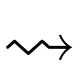
\includegraphics[height=0.4cm,width=0.4cm]{gfx/dataflow.png} 
as defined by Sattler et al. \\
It should be noted that dataflow relations, unlike structural relations, are not symmetric. 
Since we want to focus on commit regions affecting feature regions through dataflow, we designed the definitions in an according way.
Namely, we only consider interactions between a commit region $\text{r}_\text{c}$ and a feature region $\text{r}_\text{f}$, 
s.t. $\text{r}_\text{c}$ 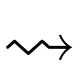
\includegraphics[height=0.4cm,width=0.4cm]{gfx/dataflow.png} $\text{r}_\text{f}$.
This choice doesn't affect the definition of structural interactions, where we want to consider both cases, since 
$\text{r}_\text{c}$ 
\includegraphics[height=0.35cm,width=0.27cm]{gfx/bigocirc.png} $\text{r}_\text{f}$ $\Leftrightarrow$
$\text{r}_\text{f}$ 
\includegraphics[height=0.35cm,width=0.27cm]{gfx/bigocirc.png} $\text{r}_\text{c}$. \\
%, as 
\includegraphics[height=0.35cm,width=0.27cm]{gfx/bigocirc.png} is a symmetric relation. \\

\begin{lstlisting}[language=C++, caption={Commit Feature Interactions}, label=DescriptiveLabel]	
1. int calc(int val) {                             %\vartriangleright% %d93dj4gr%
2.    int ret = val + 5;                           %\vartriangleright% %7shd28dj%
3.    if (FeatureDouble) {                         %\vartriangleright% %fu3w17ds%    %\vartriangleright% %FeatureDouble%
4.        ret = ret * 2;                           %\vartriangleright% %fu3w17ds%    %\vartriangleright% %FeatureDouble%
5.    }                                            %\vartriangleright% %fu3w17ds%    %\vartriangleright% %FeatureDouble%
6.    return ret;                                  %\vartriangleright% %d93dj4gr%   
7. }                                               %\vartriangleright% %d93dj4gr%   
\end{lstlisting}
The code example contains both structural as well as dataflow-based commit feature interactions.
It's obvious that commit fu3w17ds implements the functionality of FeatureDouble for this function.
It follows that a structural CFI can be found between them, as their respective commit and feature region overlap.
Commit 7shd28dj introduces a new variable that is later used inside the feature region of the "Double"-Feature. 
This accounts for a CFI through dataflow, as data that was produced within a commit region is used as input 
inside an instruction of a feature region later on in the program. \\

\textbf{Definition 8.} The occurance of structural interactions between a commit and a feature region is defined as a \textbf{structural commit-feature interaction}. \\

\textbf{Definition 9.} The occurance of dataflow interactions from a commit region to a feature region is defined as a \textbf{dataflow-based commit-feature interaction}. 

\subsection*{Implementation}\label{ch:implementation}

The detection of structural as well as dataflow-based commit-feature interactions is implemented in VaRA \cite{VaRA2023}.
Similarly to SEAL, VaRA maps information onto the compiler's IR during its construction.
This makes it possible to extract two types of information on llvm-IR instruction level. \\
The first type are code-regions, more specifically commit and feature regions as defined in definition 1. and 3.
Thus, structural commit-feature interactions can be collected by iterating over the compiled instructions of a program.
According to definition 8., we can store a structural interaction between a commit and a feature, if an instruction is part of a respective commit and feature region.
%If an instruction is part of a feature as well as a commit region, we can save a structural commit-feature interaction for them.
For each such interaction we also save the amount of instructions it occurs in. 
This is accomplished by incrementing its instruction counter if we happen to encounter a duplicate. \\
The second kind are taints, more specifically commit taints as defined in definition 2.
Similarly to commit and feature regions, VaRA allows us to extract the information of its commit taints for each instruction.
Thus, dataflow-based commit-feature interactions can also be iteratively collected on instruction level.
According to definition 9., we can store a dataflow-based interaction between a commit and a feature, if an instruction has a respective commit taint while belonging to a respective feature region.
%We save a dataflow-based interaction between a feature and a commit when an instruction is tainted by a commit while belonging to a feature region.
Consequently said instruction uses data, that was changed by a commit region earlier in the program, as its input, while stemming from code belonging a feature region. \\
For our research we examine numerous software projects to get a wide range of reference data, as commit-feature interactions could potentially vary greatly between different code spaces.
Accordingly, the VaRA-Tool-Suite was extended making it possible to generate a report comprising all found CFIs of an according type in a software project.
This aids us in examining several software projects to gain sufficient and sensible data about commit-feature interactions.
The created reports are also evaluated in the VaRA-Tool-Suite, which offers support to process and display statstics of the generated data. \\

\subsection*{Conceptualization}

Here, we introduce concepts and meanings of structural and dataflow-based commit-feature interactions as well as a combination therof.  \\
A structural interaction between a commit and a feature implies that the instruction said interaction occurs in, stems from code that was last changed by said commit and implements functionality of said feature.
It follows that the commit of the interaction contributed code to, i.e. was used to implement, the feature. 
At the same time we know that each LOC inside a git project was added and last changed by a commit. 
Thus, every instruction belonging to a feature region is also part of a commit region.
By definition, feature regions encompass the entire code space implementing the functionality of their respective features.
This means that the commits structurally interacting with a feature, are the commits constituting the code space, i.e. implementing the functionality, of said feature.
Following this, we can also say that a commit implements the features it structurally interacts with.
By accessing high-repository information, we can determine the author of each commit.
Extracting the authors of all commits a feature has structural interactions with, determines the authors that implemented it. \\ \\
We also want to introduce the concept of \textbf{feature scope} as the amount of instructions stemming from a feature's region.
The amount of instructions can simply be added up from the amount of instructions saved inside each structural interaction of a feature. 
The scope of a feature is meant to be a useful measure to assess the extend to which a feature interacts with commits.
Features with very little scope, but many dataflow interactions with commits, might be more interesting than features with large scope and the same amount of interactions. \\
For a feature, it's also possible to estimate the extend to which each of its developers contributed to its implementation.
This can be accomplished by tracing back each structural interaction of the feature with a commit, to the commit's author.
Now, adding up the amount of instructions for each author and putting it into contrast with the scope of a feature can show how much a developer contributed to the implementation of a feature. \\ \\
Instructions with structural commit-feature interactions do likely introduce or change data that will be used within the feature of that interaction.
Thus, structural interactions heavily coincide with dataflow-based interactions. 
Unlike dataflow interactions that don't coincide with structural interactions, programmers are much more aware of them.
That's why we want to be able to separate these two kinds of dataflow interactions.
This can be accomplished by simply checking whether a commit that influences a feature through dataflow, also structurally interacts with it.

